% Generated by code/ch11_tomography.py -- do not edit by hand.
\definecolor{qocA}{rgb}{0.00,0.45,0.70}
\definecolor{qocB}{rgb}{0.90,0.60,0.00}
\definecolor{qocC}{rgb}{0.00,0.62,0.45}
\definecolor{qocD}{rgb}{0.80,0.40,0.00}
\definecolor{qocE}{rgb}{0.80,0.60,0.70}
\definecolor{qocF}{rgb}{0.35,0.70,0.90}
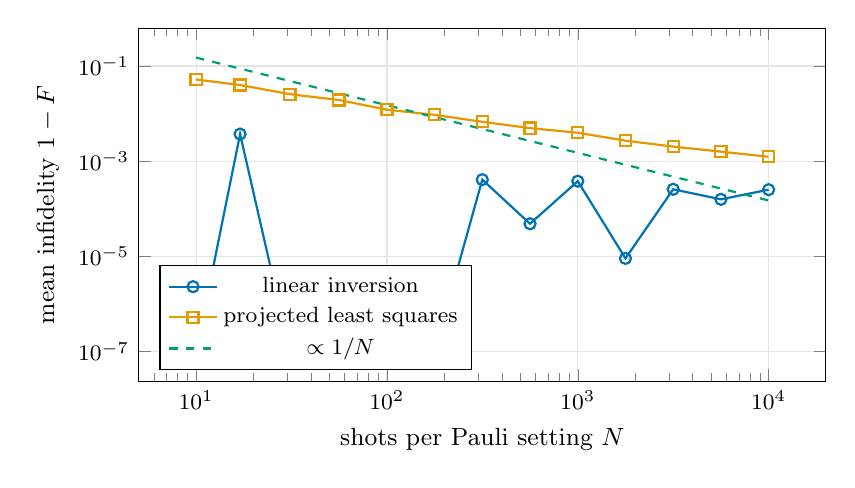
\begin{tikzpicture}[]
\begin{axis}[width=0.85\linewidth, height=0.5\linewidth, xlabel={shots per Pauli setting $N$}, ylabel={mean infidelity $1-F$}, legend pos=south west, legend style={font=\footnotesize}, tick label style={font=\footnotesize}, label style={font=\small}, grid=major, grid style={gray!20}, xmode=log, ymode=log]
\addplot[thick, qocA, mark=o] coordinates {(10,1e-07) (17,0.0037217) (31,1e-07) (56,1e-07) (100,1e-07) (177,1e-07) (316,0.0004102) (562,4.8665e-05) (1000,0.00038091) (1778,9.0958e-06) (3162,0.00025758) (5623,0.00015848) (10000,0.00025251)};
\addplot[thick, qocB, mark=square] coordinates {(10,0.05213) (17,0.039875) (31,0.025586) (56,0.019346) (100,0.01207) (177,0.0094574) (316,0.006732) (562,0.0049607) (1000,0.0039679) (1778,0.0027045) (3162,0.0020278) (5623,0.001591) (10000,0.0012428)};
\addplot[thick, qocC, dashed] coordinates {(10,0.15) (17,0.088235) (31,0.048387) (56,0.026786) (100,0.015) (177,0.0084746) (316,0.0047468) (562,0.002669) (1000,0.0015) (1778,0.00084364) (3162,0.00047438) (5623,0.00026676) (10000,0.00015)};
\legend{linear inversion, projected least squares, $\propto 1/N$}
\end{axis}
\end{tikzpicture}
